\section{Comparison of the traditional and new approaches to
compartmental modelling}

Two simulation studies are used to compare the performance of the
traditional and new compartmental models. These studies are based
on a branched model neuron with known expression for the somal
potential in response to large scale exogenous input (see Appendix
4). The first study examines the accuracy with which each type of
compartmental model estimates this somal potential, and uses the
NEURON simulator (Hines and Carnevale, \cite{Hines97}) as an
example of a traditional compartmental model. The second study
assesses the accuracy of the two types of models by comparing the
statistics of the spike train output generated by each model when
the test neuron is subjected to large scale synaptic input. Here a
traditional compartmental model developed by the authors is used.
This model gave results identical to those of NEURON in the first
study. Finally, a time step of one microsecond is used in the
numerical integration of each compartmental model to ensure that
errors in temporal integration make no significant contribution to
the error in the calculation of membrane potential.

\subsection{The test neuron}

One way to construct a branched test neuron with a closed form
solution for the somal potential is to choose the radii and
lengths of its sections such that the Rall conditions for an
equivalent cylinder are satisfied (Rall, \cite{Rall64}). These
conditions require that the sum of the three-halves power of the
diameters of the child limbs is equal to the three-halves power of
the diameter of the parent limb at any branch point, and that the
total electrotonic length from a branch point or the soma to a
dendritic tip is independent of path. The test neuron illustrated
in Figure \ref{TestNeuron} satisfies these conditions. When the
Rall conditions are satisfied, the effect at the soma of any
configuration of input on the branched model of the neuron is
identical to the effect at the soma of the unbranched equivalent
cylinder with biophysical properties and configuration of input
determined uniquely from those of the original branched neuron
(Lindsay \emph{et al.}, \cite{Lindsay03}).

\begin{figure}[!h]
\[
\begin{array}{c}
$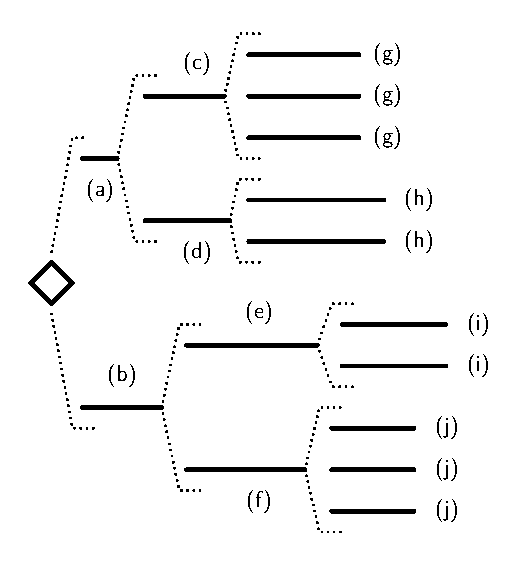
\includegraphics[ ]{NCFig4.eps}$
\end{array}\qquad
\begin{array}{ccc}
\hline
\mbox{Section} & \mbox{Length }\mu\mbox{m} & \mbox{Diameter }\mu\mbox{m}\\[2pt]
\hline
 (a) & 166.809245 & 7.089751 \\
 (b) & 379.828386 & 9.189790 \\
 (c) & 383.337494 & 4.160168 \\
 (d) & 410.137845 & 4.762203 \\
 (e) & 631.448520 & 6.345604 \\
 (f) & 571.445800 & 5.200210 \\
 (g) & 531.582750 & 2.000000 \\
 (h) & 651.053246 & 3.000000 \\
 (i) & 501.181023 & 4.000000 \\
 (j) & 396.218388 & 2.500000 \\
\hline
\end{array}
\]
\centering
\parbox{5in}{\caption{\label{TestNeuron} A branched neuron
satisfying the Rall conditions. The diameters and lengths of the
dendritic sections are given in the right hand panel of the
figure. At each branch point, the ratio of the length of a section
to the square root of its radius is fixed for all children of the
branch point.}}
\end{figure}

%\begin{figure}[!h]
%\[
%\begin{array}{c}
%$\begin{mfpic}[1][1]{0}{220}{-20}{220}
%\pen{2pt}
%\dotsize=1pt
%\dotspace=3pt
%\lines{(-5,100),(5,110),(15,100),(5,90),(-5 ,100)}
%% Upper dendrite
%% Root branch
%\dotted\lines{(5,115),(15,170),(20,170)}
%\lines{(20.0,160),(36.7,160)}
%\tlabel[tc](28.4,150){\textsf{(a)}}
%% Level 1
%\lines{(50.0,190),(88.3,190)}
%\tlabel[bc](75,200){\textsf{(c)}}
%\lines{(50.0,130),(91.0,130)}
%\tlabel[tc](75,120){\textsf{(d)}}
%\dotted\lines{(36.7,160),(45,200),(55,200)}
%\dotted\lines{(36.7,160),(45,120),(55,120)}
%% Level 2
%\lines{(100.0,210),(153.2,210)}
%\lines{(100.0,190),(153.2,190)}
%\lines{(100.0,170),(153.2,170)}
%\tlabel[cl](160,210){\textsf{(g)}}
%\tlabel[cl](160,190){\textsf{(g)}}
%\tlabel[cl](160,170){\textsf{(g)}}
%\dotted\lines{(88.3,190),(95,220),(105,220)}
%\dotted\lines{(88.3,190),(95,160),(105,160)}
%\lines{(100.0,140),(165.1,140)}
%\lines{(100.0,120),(165.1,120)}
%\dotted\lines{(91.0,130),(95,150),(105,150)}
%\dotted\lines{(91.0,130),(95,110),(105,110)}
%\tlabel[cl](175,140){\textsf{(h)}}
%\tlabel[cl](175,120){\textsf{(h)}}
%%
%% Lower dendrite
%% Root branch
%\lines{(20.0,40),(58.0,40)}
%\dotted\lines{(5,85),(15,30),(25,30)}
%\tlabel[bc](39,50){\textsf{(b)}}
%% Level 1
%\lines{(70.0,70),(133.1,70)}
%\lines{(70.0,10),(127.1,10)}
%\dotted\lines{(58,40),(66.5,80),(76.5,80)}
%\dotted\lines{(58,40),(66.5,0),(76.5,0)}
%\tlabel[bc](105,80){\textsf{(e)}}
%\tlabel[tc](105,0){\textsf{(f)}}
%% Level 2
%\lines{(145,80),(195.1,80)}
%\lines{(145,60),(195.1,60)}
%\dotted\lines{(133.1,70),(140,90),(150,90)}
%\dotted\lines{(133.1,70),(140,50),(150,50)}
%\tlabel[cl](205,80){\textsf{(i)}}
%\tlabel[cl](205,60){\textsf{(i)}}
%\lines{(140,30),(179.6,30)}
%\lines{(140,10),(179.6,10)}
%\lines{(140,-10),(179.6,-10)}
%\dotted\lines{(127.1,10),(134,40),(144,40)}
%\dotted\lines{(127.1,10),(134,-20),(144,-20)}
%\tlabel[cl](190,30){\textsf{(j)}}
%\tlabel[cl](190,10){\textsf{(j)}}
%\tlabel[cl](190,-10){\textsf{(j)}}
%\end{mfpic}$
%\end{array}\qquad
%\begin{array}{ccc}
%\hline
%\mbox{Section} & \mbox{Length }\mu\mbox{m} & \mbox{Diameter }\mu\mbox{m}\\[2pt]
%\hline
% (a) & 166.809245 & 7.089751 \\
% (b) & 379.828386 & 9.189790 \\
% (c) & 383.337494 & 4.160168 \\
% (d) & 410.137845 & 4.762203 \\
% (e) & 631.448520 & 6.345604 \\
% (f) & 571.445800 & 5.200210 \\
% (g) & 531.582750 & 2.000000 \\
% (h) & 651.053246 & 3.000000 \\
% (i) & 501.181023 & 4.000000 \\
% (j) & 396.218388 & 2.500000 \\
%\hline
%\end{array}
%\]
%\centering
%\parbox{5.5in}{\caption{\label{TestNeuron} A branched neuron
%satisfying the Rall conditions. The diameters and lengths of the
%dendritic sections are given in the right hand panel of the
%figure. At each branch point, the ratio of the length of a section
%to the square root of its radius is fixed for all children of the
%branch point.}}
%\end{figure}

The high degree of accuracy used in the specification of the
dendritic radii and section lengths of the test neuron is required
to ensure that the equivalent cylinder is an adequate
representation of the test neuron. The membrane of the test neuron
is assigned a specific conductance of $0.091\,$mS/cm$^2$
($g_\mathrm{M}$) and specific capacitance of $1.0\,\mu$F/cm$^2$
($c_\mathrm{M}$), and has axoplasm of conductance $14.286\,$mS/cm
($g_\mathrm{A}$). With these biophysical properties, the
equivalent cylinder has length one electrotonic unit. The soma of
the test neuron is assumed to have membrane area $A_\mathrm{S}$,
and specific conductance $g_\mathrm{S}$ and specific capacitance
$c_\mathrm{S}$ identical to that of the dendritic membrane. The
analytical expression for its somal potential is given in Appendix
4.
